\chapter{Automatic Memory Management}

Programs need physical memory to store their data. Between the idealized runtime representation of data in a high-level language and the actual physical, localized storage we find several layers of indirection. For the purpose of this chapter we will take the memory management provided by the Operating System as a given and build on top of it to provide memory to \rift programs.

\section{Problem Statement}

Considering the simple C++ program given in \autoref{lst:mem-cpp} we can observe various strategies on how to store program state.

\begin{lstlisting}[language=cpp, caption={Memory in C++}, label={lst:mem-cpp}]
void aFunction() {
  int i = 0;
  Vector b(1, 2, 3);
  Vector * c = new Vector(1, 2, 3);
  globalVector = c;
}

void main() {
  aFunction();
  delete globalVector;
}
\end{lstlisting}

The first allocation on line 2 is trivial to translate, since it conveniently maps without further complications to a machine register. The Vector $b$ created on line 3 is a bit more complicated. C++ semantics dictate that the vector is not to be accessed after the closing bracket on line 6, \ie we say it goes out of scope. A natural choice for a compiler would be to store it inside the current activation frame of the runtime stack. Finally $c$ created on line 4 is allocated using the $new$ operator. Hereby we request the compiler to allocate it in a more permanent fashion, so we can reuse it outside the current function scope.

\begin{figure}[h]
\centering
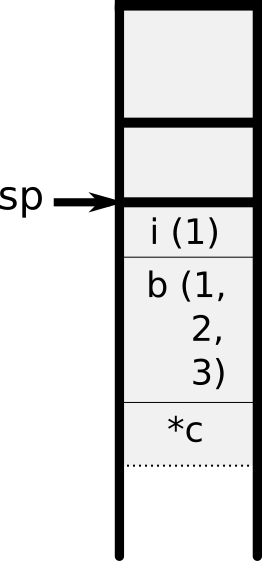
\includegraphics[width=0.2\textwidth]{runtime_stack}
\caption{Runtime stack when aFunction from \autoref{lst:mem-cpp} is activated.}
\label{fig:runtime-stack}
\end{figure}

A possible choice for an activation frame of aFunction from \autoref{lst:mem-cpp} is given in \autoref{fig:runtime-stack}. Assuming the variable $i$ had to be stored permanently at some point we can see the value of i and the contents of the vector $b$ stored inside the current frame. Note that to release all the memory upon returning from the function it suffices to adjust the stack pointer (SP). This allows us to reuse the memory without further overhead. Finally the variable $c$ is not stored on the stack, rather we only keep a pointer (denoted $*c$) and store the actual value outside the stack. We call this \emph{heap allocation}. Storage allocated on the heap is not reclaimed by returning from the function. This allows us to use the value in a higher up, \ie earlier frame; or as we can see in \autoref{lst:mem-cpp} on line 5 to assign it to a global value. In C++ heap objects are not automatically reclaimed and the programmer is responsible to manually delete the object when its no longer in use.

It might seem that we could write most programs to just use heap allocated memory and thereby avoid the cognitive overhead of requesting and releasing memory. In practice most programming languages would want to provide heap storage to the user. In particular stack allocated memory is

\begin{description}
  \item[limited] The runtime stack needs to be a linear address space which is more expensive to provide than a segmented address spaces.
  \item[local] We might be allowed to pass references to values inside our own call frame to later frames, but it will never be possible to return a reference. Thus all return values need to passed by value, \ie copied down to the previous function which is expensive.
\end{description}

\subsection{Allocation Sites in \rift Code}

If we consider \rift code the situation is a bit different. Lets consider the code in \autoref{lst:mem-rift} and the corresponding memory which is allocated as shown in \autoref{fig:rift_stack}.

\begin{lstlisting}[language=rift, caption={Some values allocated in \rift.}, label={lst:mem-rift}]
function(a) {
  b <- 1
  b <- a + b
}
\end{lstlisting}

\begin{figure}[h]
\centering
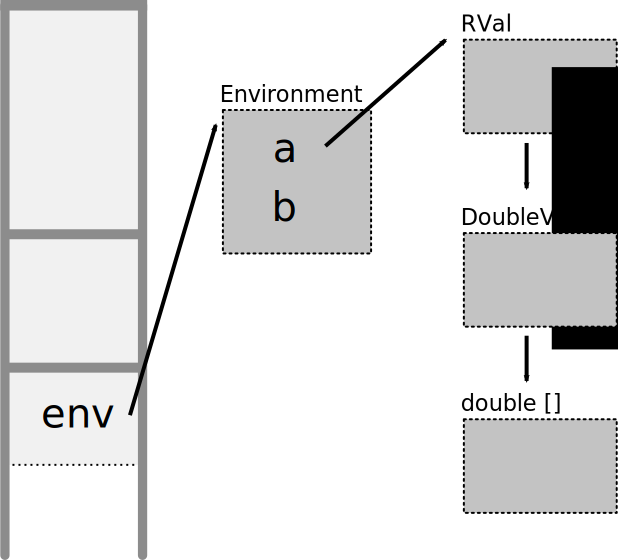
\includegraphics[width=0.5\textwidth]{rift_stack}
\caption{Memory layout of a \rift function given in \autoref{lst:mem-rift}.}
\label{fig:rift_stack}
\end{figure}

Unlike in the C++ case all \rift values are allocated on the stack. This releases the programmer from the cognitive burden to figure out where to put its values. In the spirit of a dynamic language he can pass any value to any function and of course also return it. The runtime stack is only used to keep track of environments, which are the runtime representation of \rift stack frames.

Of course this creates a problem. As demonstration we run a very simple \rift program given in \autoref{lst:rift-mem-usg}. 

\begin{lstlisting}[language=rift, caption={loop.ri}, label={lst:rift-mem-usg}]
a <- 100000
b <- 1
while(a > 0) {
  b <- b + a
  a <- a - 1
}
b
\end{lstlisting}

We can record the memory usage of this program using the \emph{massif} tool of \emph{valgrind} as shown in \autoref{lst:massif}.

\begin{lstlisting}[language=bash, label={lst:massif}]
valgrind --tool=massif ./rift loop.ri
\end{lstlisting}

\emph{Massif} writes a log file of all allocations. We visualize it with the massif-visualizer tool. As we can see in \autoref{fig:massif-blowup} the heap size grows unbounded even though a constant amount of memory would be enough to hold all state of the code in \autoref{lst:rift-mem-usg}. It becomes very obvious that all our runtime functions, \eg $doubleGt$ or $genericAdd$ leak all memory they allocate.

\begin{figure}[h]
\centering
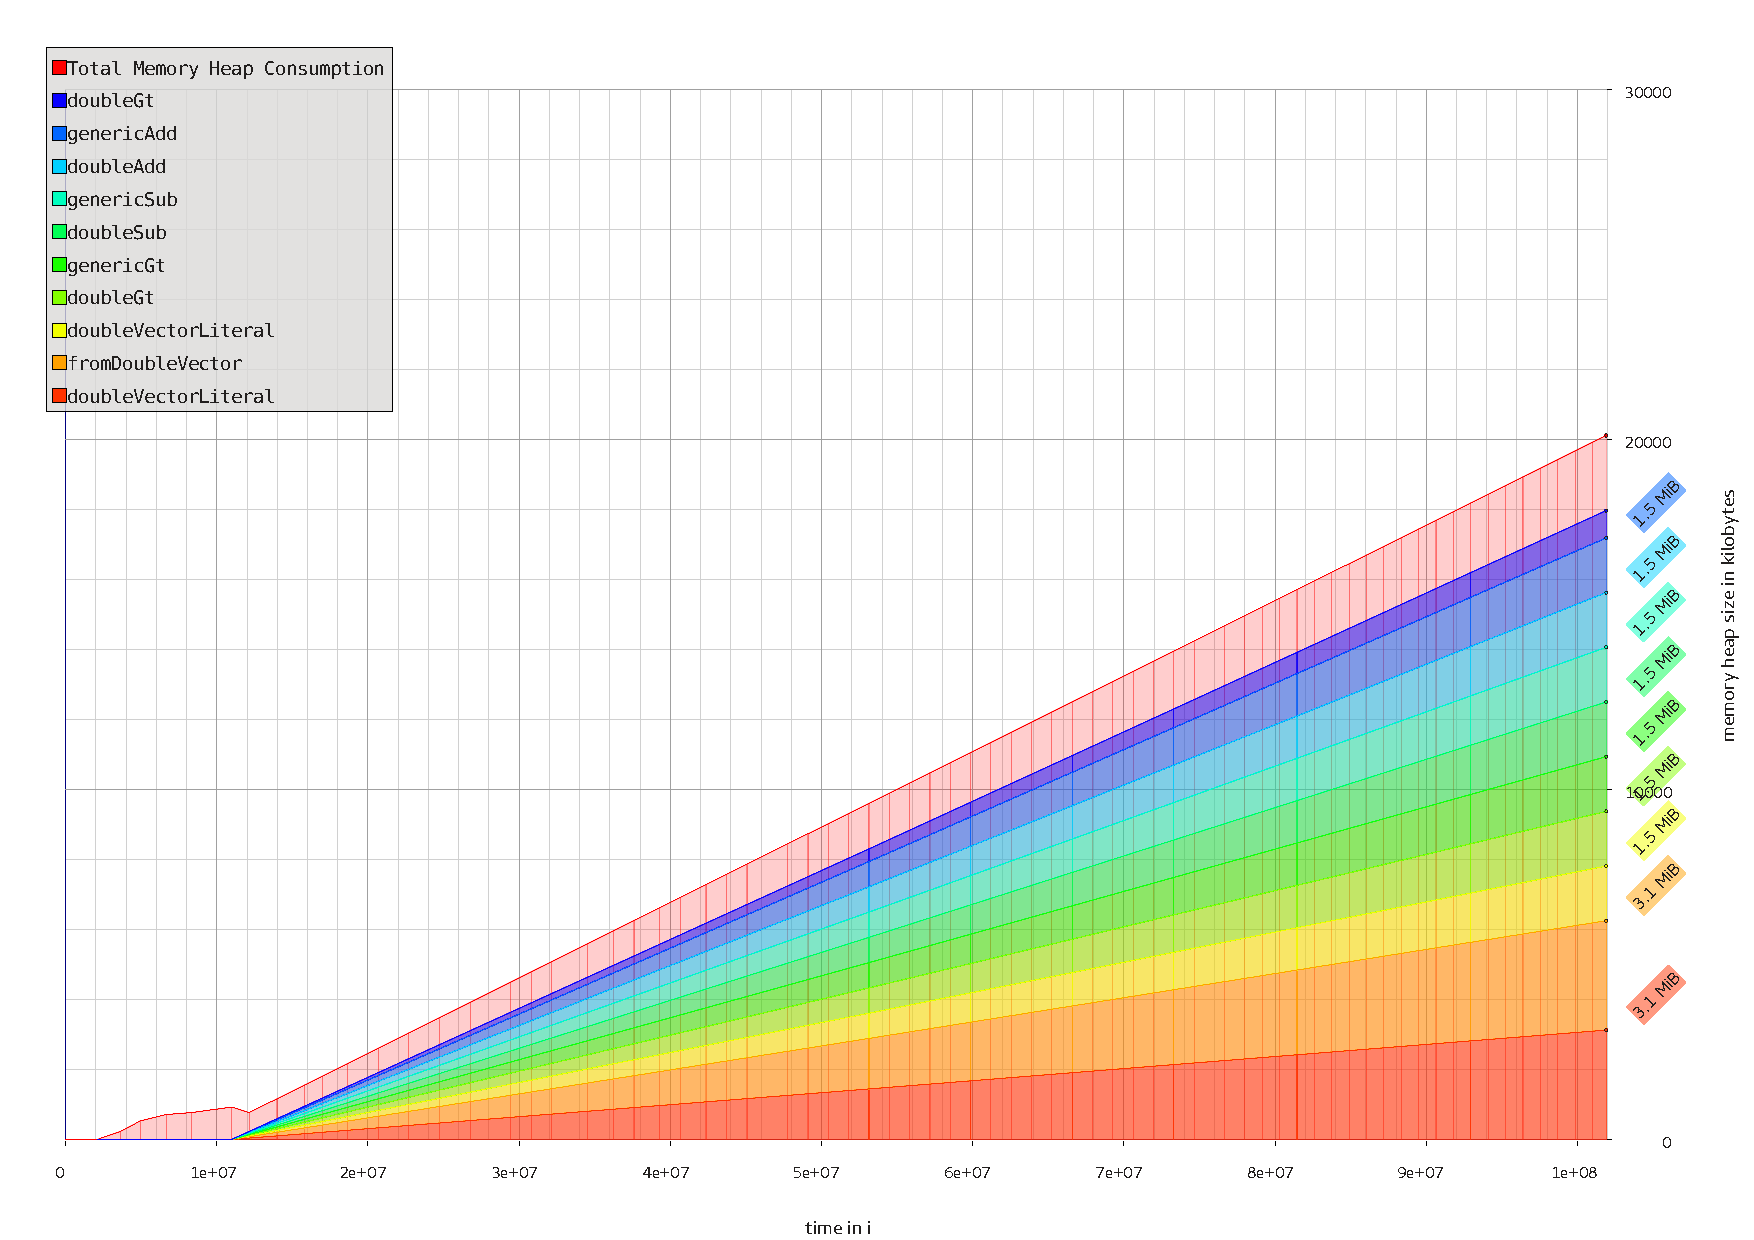
\includegraphics[width=1\textwidth, height=1\textwidth]{massif-blowup}
\caption{Memory consumption of a \rift program given in \autoref{lst:rift-mem-usg} without any memory management enabled.}
\label{fig:massif-blowup}
\end{figure}

The natural question arises of how to deal with the problem. We could be tempted to introduce the delete operation into the \rift language. This would probably be quite hard to achieve: Many \rift statements implicitly allocate as a side effect and we never really get hold of the allocated memory. Consider \eg the $if$ statement, which will evaluate the boolean value of the condition. \Rift semantics require this comparison to allocate a numerical result vector. It would be quite unpleasant to have to clean up all those implicitly created vectors explicitly. Thus we will evaluate our options in the following chapters.

\section{Strategies}

In our language we want to be able to run programs for a long time without unnecessarily running out of memory. But on the other hand we do not want the programmer to be bothered with keeping track of allocations.

Therefore we will design the system in a way which causes all unused memory to be reclaimed automatically without user intervention. There are quite a few options available which we will discuss.

\subsection{Type System Based}

We could try to determine the lifetime of all objects in our system at compile time. There are some recent advances in this direction. E.g. the \emph{rust} language uses a notion of ownership. Every object has to be owned by another one, and it will be automatically removed when its owner gets removed. \emph{Rust} features a type system employing ownership types to statically enforce correct behavior. Whenever you want to pass an object around you have to explicitly transfer its ownership.

While this is certainly a nice approach, in the spirit of our dynamic, low cognitive overhead, easy on the programmer language we do however not want to bother the programmer with figuring out the ownership relations between his objects. We must therefore look at ways to clean up the memory at runtime.

\subsection{Reference Counting}

A simple technique employed by many language implementations is called \emph{reference counting}. The core idea is to count the number of references existing in the system for every object. When we assign the same value to a second variable the counter increases. When a reference goes out of scope it decreases. When the counter goes to zero the object is no longer used and can be removed.

While simple this idea has several drawbacks. First of all it introduces a fairly high runtime overhead to the program. Updating as well as looking up the counters is expensive. Second the technique is not able to free objects if they have cyclic references. Consider a group of several dead objects -- completely unreachable from the current program state -- but \eg placed in a circular buffer. Since they all point to the next object the circle closes and each of them has a reference count of one and will therefore not be freed.

\subsection{Tracing Garbage Collector}

Instead of keeping track of all the dependencies all the time the idea of \emph{tracing garbage collection} -- sometimes referred to as just \emph{garbge collection} (GC) -- is to only interrupt when running out of memory. At the core we have the following (conservative) assumption:

\emph{Everything which is reachable is still used}.

\begin{description}
  \item[Why is is conservative?] Sometimes programs -- either because of the scoping rules of the language or because of programming errors -- keep references to objects which they don't use anymore.
  \item[Is the assumption sound?] Depending on the language. Some languages feature raw pointers and a program might read/write to computed memory locations. E.g. in a C++ program it is possible to reconstruct a pointer from an arithmetic operation like: $(int*)(i+20)$. In \rift however the assumption is sound since all references are managed by the VM.
\end{description}

On a side note it might be interesting to ask what kind of runtime overhead GC introduces. It is almost impossible to come up with a simple measurement since it heavily depends on the workload, on the language, on the implementation of the language and so on. In practice an overhead between a few percents and up to 20 percent are observed, even in well tuned implementations.

Before we look at some algorithms to perform a GC let us define the notion of reachability in a more precise way.

\subsection{Reachability}

Let $b$ be called \emph{reachable in one step from} $a$, written as $a \rightarrow^{1} b$, \emph{iff} $a$ denotes an object containing a reference to the object $b$. We call $b$ \emph{reachable from} $a$, written as $a \rightarrow^{*} b$, \emph{iff} $\exists c_1 ... c_n : a \rightarrow^{1} c_1 \rightarrow^{1} ... \rightarrow^{1} c_n \rightarrow^{1} b$, \ie we define reachability as the transitive closure of having a reference to an object. Finally we call an object $b$ reachable, written as $\rightarrow^{*} b$ \emph{iff} $R \rightarrow^{*} b$ where $R$ denotes the \emph{root set} of live objects.

In a typical environment the \emph{root set} contains \eg global variables, symbols, events and prominently \emph{all the pointers on the runtime stack}. The stack potentially contains temporary values which do not have an assigned name, are not stored in any object yet, but will be used by later instructions. We are therefore often required to assume every pointer on the runtime stack to be part of the root set.

\subsection{Timing}

In the context of the GC we call the running program the mutator, since it is mutating the object graph outside the GC control. We define a \emph{stop the world GC} to be a one which completely halts all mutator threads, then performs the GC and finally resumes the mutator. As we see in \autoref{fig:gc_timing} another option is to run certain parts of GC concurrent to the program. In this case we need to ensure that the collector does not interfere with the mutator and that the mutator does not invalidate the work already done by the collector in an unsafe way.

\begin{figure}[h]
\centering
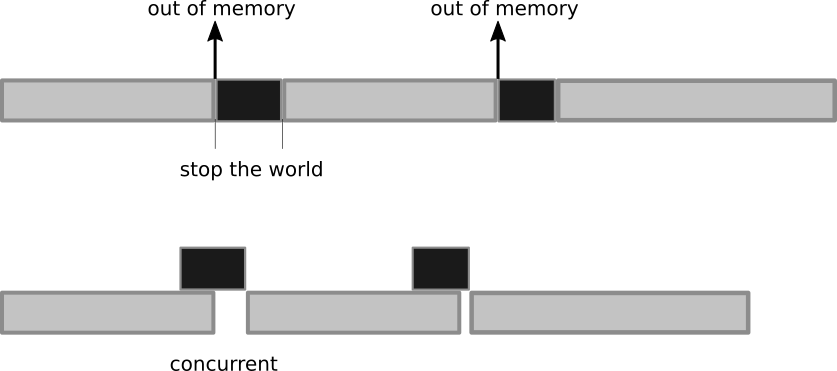
\includegraphics[width=0.6\textwidth]{gc_timing}
\caption{In its simplest form the program execution (gray) is completely stopped while the GC (black) is running. More advanced would be to let certain parts of the GC run in parallel to the normal program.}
\label{fig:gc_timing}
\end{figure}

\subsection{Strategies}

Finally we are ready to look at two representative GC algorithms.

\subsection{Stack Pointers}
\subsection{Conservative Marking}

\section{\Rift implementation}
